\chapter{Ausgangslage und Zielstellung}\label{cha:Ausgangslage und Zielstellung}

Die in diesem Bericht dokumentierte Auslegung, beschäftigt sich mit dem Tragflügel des studentischen AUVSI Flugzeugs welches im Labor für Systemtechnik entwickelt wurde. Die vorangegangenen Flugzeuggenerationen und das Reglement der Wettbewerbs bilden die Ausgangslage für die Weiterentwicklung.

\section{Historie des AUVSI SUAS-Wettbewerbs}
Seit 2002 findet jährlich der AUVSI (Association for Unmanned Vehicle Systems International) SUAS (Student Unmanned Aerial Systems Competition)-Wettbewerb in den USA statt.

Hieran hat das studentische Hochschulteam in den Jahren 2015 und 2016 erfolgreich teilgenommen. Bereits im Jahr 2014 gab es die ersten Anstrengungen ein für diesen Wettbewerb passende Flugplattform zu entwickeln. Leider war dies zu diesem Zeitpunkt noch nicht von Erfolg gekrönt. Detaillierte Informationen hierzu können der Diplomarbeit von Herrn Dipl. Ing. Fabian Meilinger entnommen werden \cite{Meiling}.

Die meisten Anforderungen an die Flugplattform ergeben sich aus dem Reglement dieses studentischen Wettbewerbs. 

\clearpage

\section{Das Flugzeug des AUVSI SUAS Teams}

Seit den ersten Erfahrungen in der Saison 2014 folgt der Konzeptionelle Aufbau des Flugzeugs demselben stark modularen Konzept. Damit wurde mit klaren Schnittstellen zwischen den Baugruppen eine getrennte Weiterentwicklung der Einzelkomponenten möglich. Dadurch enstanden beispielsweise 2015 Variationen für die Forschungsmission im Regenwald Ecuadors bei der eine deutlich Voluminösere Nutzlast mitgeführt wurde \cite{Niclas}.

\begin{figure}[H]
\centering
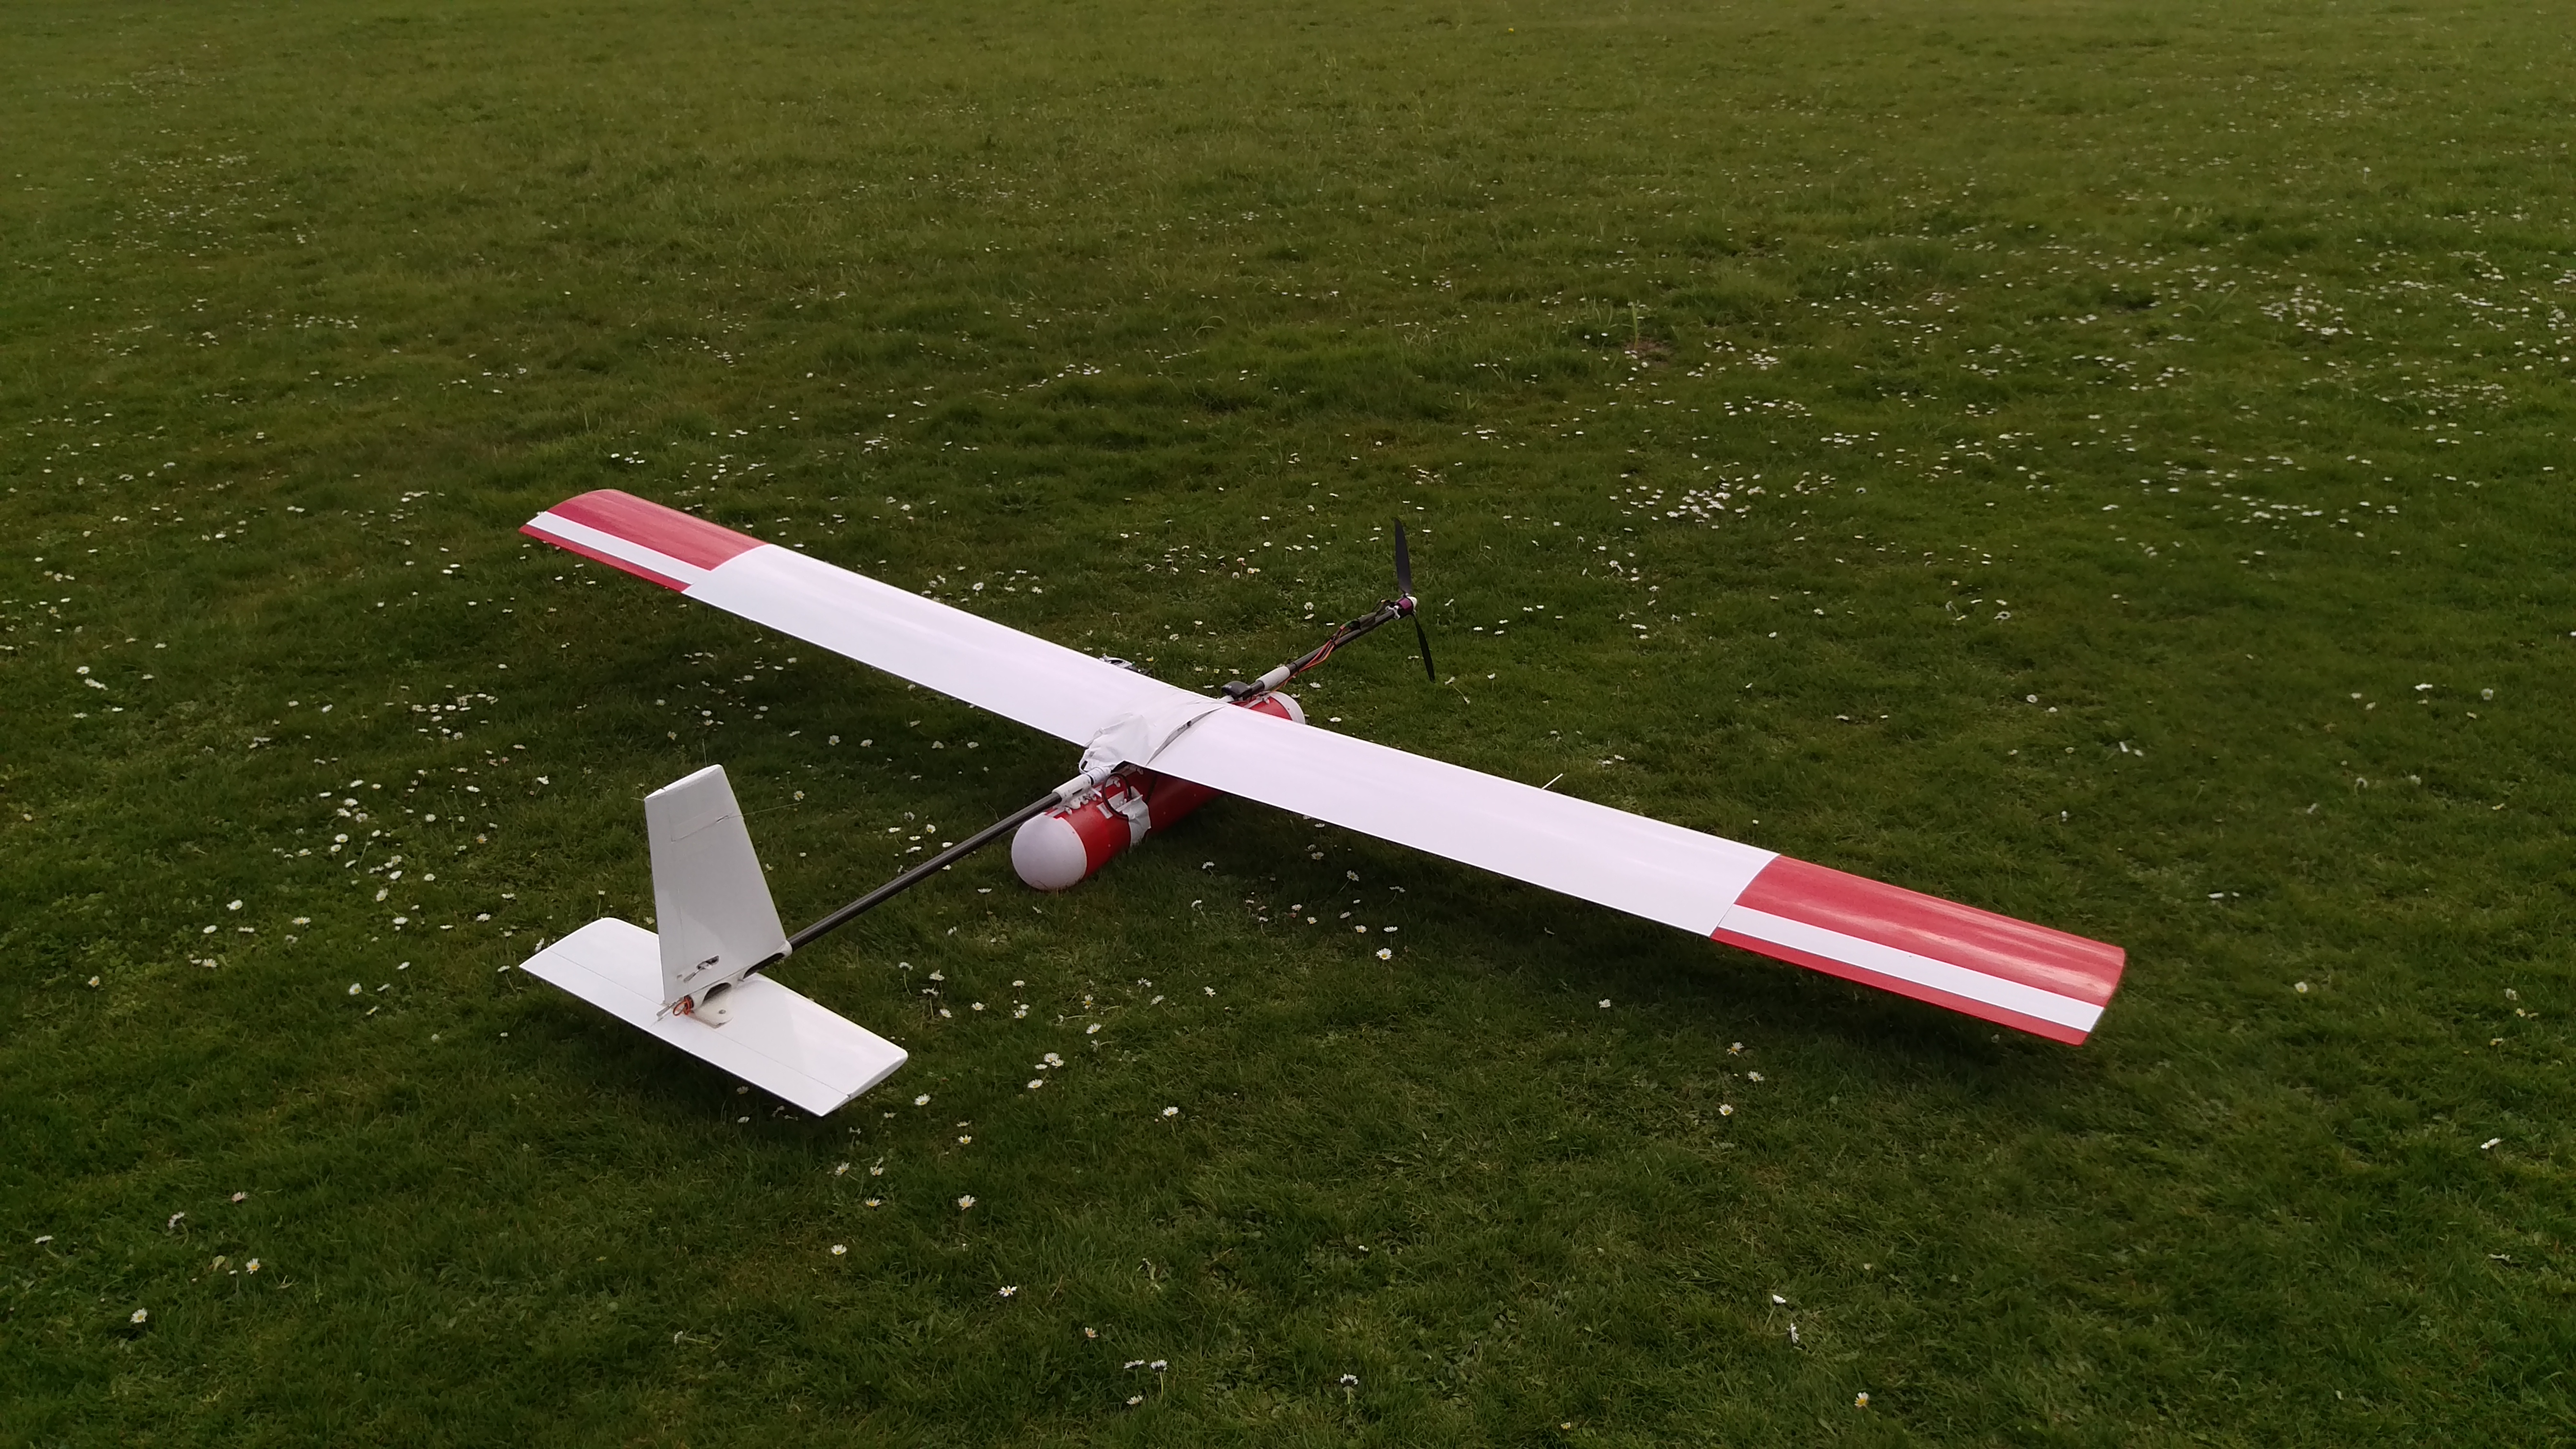
\includegraphics[width=0.9\textwidth]{bilder/Fotos/AUVSI_2015.jpg} 
\caption{Das AUVSI 2015 Modell im Einsatzzustand am Testflugplatz} 
\label{fig:Das AUVSI 2015 Modell in Einsatzzustand am Testflugplatz}
\end{figure}

Im Bild \ref{fig:Das AUVSI 2015 Modell in Einsatzzustand am Testflugplatz} ist der Gesamtaufbau des Flugzeugs zu sehen. Bisher sind der Einsatz von Rechteckigen Auftriebsflächen und Leitwerken sowie CFK-Rohren als Ausleger für Heck und Motorträger charakteristisch. Unter dem Zentralen Rumpfrohr ist der Zylinderförmige Nutzlastbehälter Montiert.


\clearpage


\section{Bisherige Flügelbauweise}

Die bisherigen Tragflügel sowie einige Leitwerksflächen wurden einer Bauweise ausgeführt die in Modellbaukreisen als "Styro-Abachi" bekannt ist. In der konkreten Variante wurde beim den AUVSI Flächen ein Kern aus Polystyrol im Querschnitt des verwendeten Clark-Y Profils mit der 4-Achs CNC Heißdrahtschneidemaschine gefertigt. In diesem Rohling wurden anschließend die Ausschnitte für Kabelschächte und die Servo Rudermaschinen eingebracht. Anschließend wurde auf der Ober und danach auf der Unterseite der Fläche mit Unterdruck im Vakuumsack eine Schicht aus 0,6 mm Abachi Funier aufgeklebt.
Anschließend wurde an den beiden Ende eine Endrippe aus 3 mm starkem Ceibasperrholz Aufgebracht. Die Kraftübertragung in die Anschließenden Segmente wurde mit in den Polystyrolblock eingeklebten CFK-Rohren realisiert.
Anschließend erfolge das Auskasten und Anschlagen der Ruderflächen.
Abschließend wird die Fläche mit Heißklebender Kunststoffolie bebügelt um sie resistent gegen Umwelteinflüsse zu machen.

Bei dieser Bauweise werden die Zugspannungen vom Aufgebrachen Abachi Funier in Faserrichtung aufgenommen. Der Polystyrolkern überträgt die Schubspannungen zwischen Ober- und Unterseite der Fläche und nimmt entstehenden Druck quer zur Oberfläche auf.
Der Begrenzende Fertigungsparameter bei der Belastung auf Biegung ist hier die Festigkeit des Klebers zwischen der Oberen (Druck) Funierlage und dem Polystyrolkern. Ein Abschälen führt zu einem Druckbeulen der Oberseitigen Funierlage und damit zum Stabilitätsversagen.

Insgesamt hat sich diese Bauweise als sehr Robust und für alle Flugsituationen ausreichend in der Stabilität erwiesen.
Die Formtreue des Profilquerschnitts ist vergleichsweise hoch, ein korrekt gefertigtes Werkzeug für die Vakuumtechnik vorrausgesetzt. 

Nachteilig sind das Vergleichsweise hohe Gewicht von 2,145\,$Kg/m^2$ [AUVSI/Ecuador 2015].
Auch beinhaltet die Fertigung einfachen Werkzeugbau und zahlreiche Handarbeitsschritte. Damit variiert das Ergebnis je nach Erfahrung und Sorgfalt des Personals deutlich. Ein Fehler beim Vakuumverkleben der Funierschicht kann die gesamte Fläche unbrauchbar machen. 

Bisher ist keine Vorauslegung und Dimensionierung der Struktur für die erwarteten Lasten durchgeführt worden.

Erfahrungen beim Versuch alte Flächen dieser Bauweise zu verschrotten, lassen erwarten das diese Flügel bisher bedeutend zu stabil und schwer gebaut worden sind. 

\clearpage

\section{Verbesserungsziele}

Die in dieser Arbeit durchgeführte Auslegung hat eine Reihe von Verbesserungen gegenüber der Jetzigen Bauform zum Ziel:
\begin{itemize}
    \item Erstellung eines Nachweises der Festigkeit der Fläche mit klar bekannten Sicherheiten und Lastgrenzen.
    \item Reduzierung des Flächengewichts durch höheren Ausnutzungsgrad der Materialwerte.
    \item Nach Möglichkeit Reduzierung des Anteils an anspruchsvoller Handarbeit und Steigerung des Anteils Mechanisierter und Werkzeugbasierter Fertigung.
    \item Nach Möglichkeit Einsatz einer weiterhin Profiltreuen Bauweise bis mindestens 25\% der Flächentiefe.
    \label{lst:Verbesserungsziele}
\end{itemize}


\section{Optimierungsgrenzen durch den Einsatz}

Die Optimierung des Flügels in Bauform und Materialwahl nach in \ref{lst:Verbesserungsziele} genannten Maßgaben ist durch eine Reihe von Situationen im Alltagseinsatz des Fluggeräts begrenzt, welche über den Statischen Flugzustand hinausgehen.

Das Fluggerät wird im Normalfall von einer kurzen Rampe mit einem Gummiseil im Flitschenstart gestartet. Dadurch entstehen kurzzeitig Lastvielfache von bis zu 3,5 g in X Richtung bis kurz über die Festgelegt Mindestfluggeschwindigkeit.
Auch ein Hochstart wurde für Einsätze in denen der Energieverbauch zum erreichen der Missionshöhe einen hohen Anteil hat an der Gesamtflugaufgabe hat disskutiert. 
Dadurch muss die Tragfläche kurzzeitig eine deutlich höheren Auftriebswert ertragen als für den Statischen Reiseflug vorgesehen. 